Now that we earned our crypto assets, let us see how we can use it in real life. I will provide some use cases, in reality there is so much you can do with crypto even there is online casinos.

\section{Converting crypto to fiat currency}

In South Africa, the main currency is the South African Rand (R). We have a main crypto exchange called Luno.

When i drove to Cape Town CBD I saw the Luno building.

\begin{figure}[H]
\centering
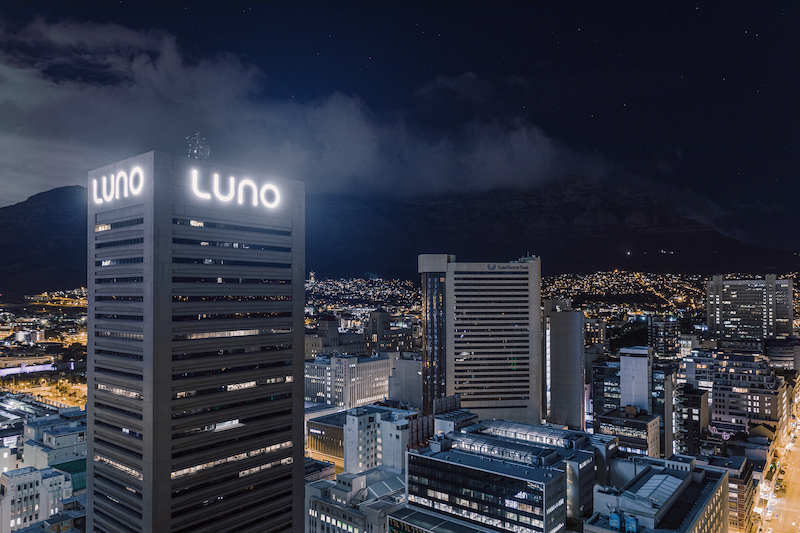
\includegraphics[width=0.8\textwidth]{Lunos-iconic-South-Africa-building-on-Cape-Towns-foreshore-district.jpg}
\caption{Luno cryptocurrency exchange skyscraper in South Africa}
\label{fig:luno}
\end{figure}

Assumptions: Let us say we mined our currency in NiceHash. \\

We move the crypto from NiceHash to Luno by doing a crypto transfer. Some network fees might be involved.

Then from Luno to our local bank account. (Note Luno captures your ID Number) I think they submit reports to SARS on its clients.

\section{Using crypto in stores}

Methodology: We use bitrefill to convert our crypto into a cash voucher.

Note: NiceHash dont capture our ID number to create a wallet nor does bitrefill. Interesting!

You can use the bitrefill website to purchase stuff from selected stores. Converting $x$ BTC or other coins to a cash voucher to its provided store.

I will show you a screenshot of the bitrefill website.

\begin{figure}[H]
\centering
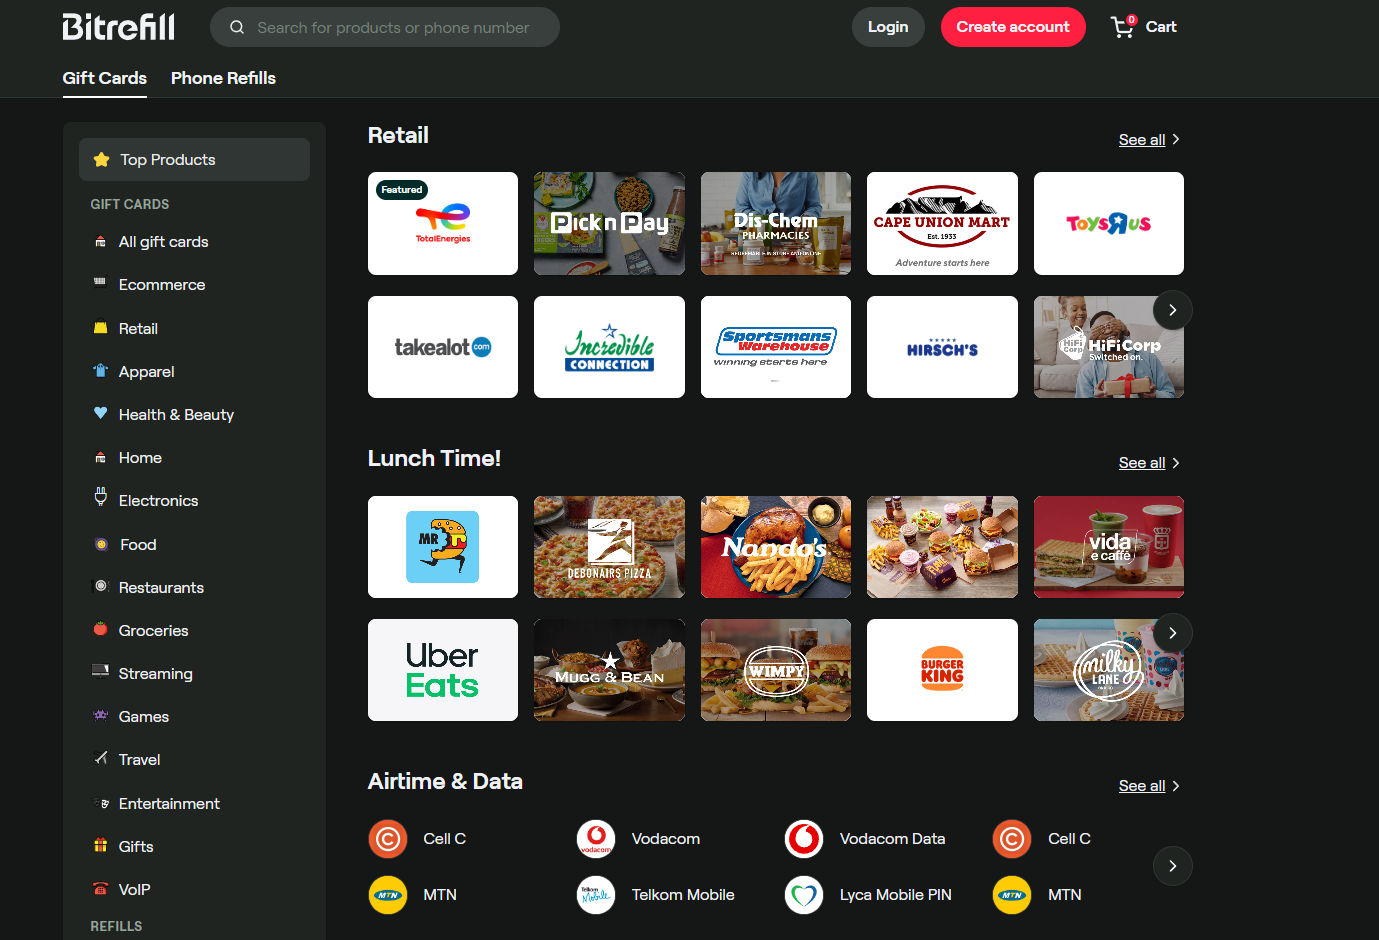
\includegraphics[width=0.8\textwidth]{bitrefill.png}
\caption{Bitrefill website}
\label{fig:bitrefill}
\end{figure}

I did try it to buy airtime for my MTN phone number also i bought a item from amazon which i will attach below.

\begin{figure}[H]
\centering
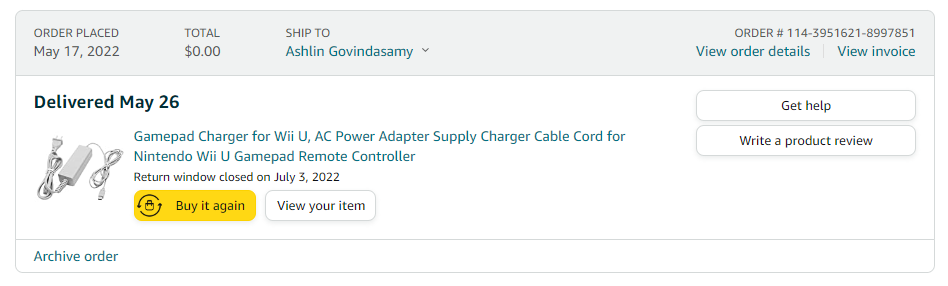
\includegraphics[width=1\textwidth]{wiiu.png}
\caption{Amazon Purchase}
\label{fig:amazon}
\end{figure}

I would try to purchase my fuel next using crypto its quite cool.

\section{Crypto Visa Card}
Crypto.com is a crypto exchange. They give customers who has $x$ amount of money with them a crypto visa card. If you would like to use your crypto in stores you can use the crypto.com visa card.

\begin{figure}[H]
\centering
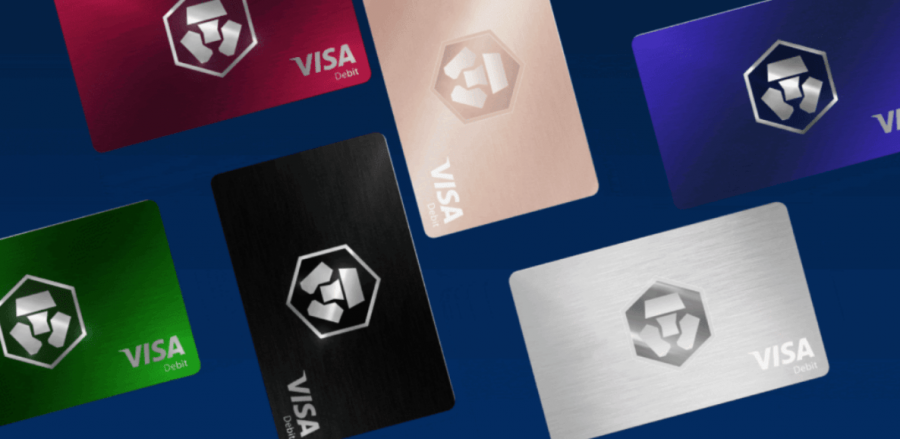
\includegraphics[width=0.5\textwidth]{how-does-it-work-900x439.png}
\caption{Crypto.com Visa card}
\label{fig:crypto}
\end{figure}

\section{Crypto ATM's}

Crypto ATM's are very cool. They allow you to convert cryptocurrencies to fiat physical cash currency conversely they allow you to convert fiat currency to cryptocurrencies. 

Around South Africa there are some Crypto ATM's in cities.

\begin{figure}[H]
\centering
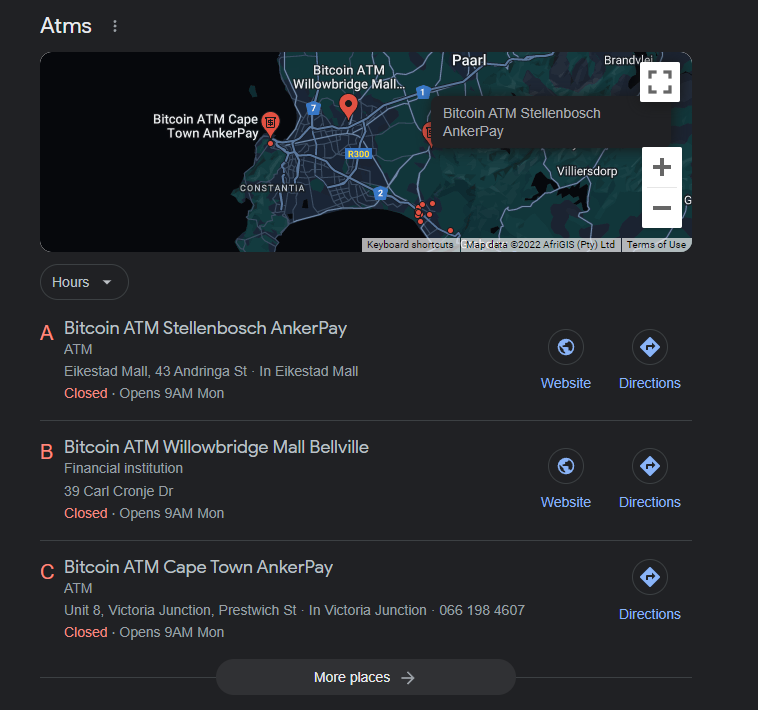
\includegraphics[width=0.5\textwidth]{cryptoatm.png}
\caption{Crypto ATM's around Cape Town}
\label{fig:crypto-atm}
\end{figure}

\begin{figure}[H]
\centering
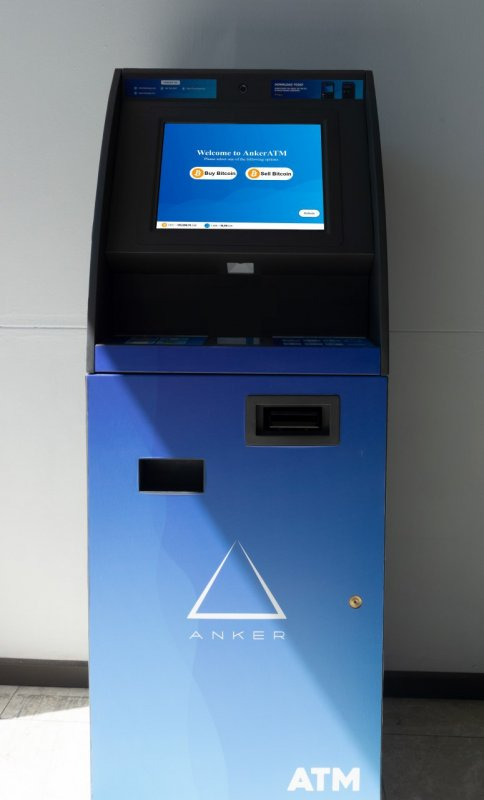
\includegraphics[width=0.5\textwidth]{ankerpay_bitcoin_atm_1c27477524.jpg}
\caption{Ankerpay ATM in Stellenbosch}
\label{fig:ankerpay}
\end{figure}

\section{Using crypto to do debit order investments}
Let us assume you pay for a debit order at $ABC$ Investments per month.

We could write a script to automate this. Lets say end of the month we need $x$ amount to pay the $x$ amount debit order investment amount.

Two places offer APIs to transfer crypto funds.

\begin{itemize}
\item Luno
\item NiceHash
\end{itemize}

Psuedo code:

\begin{verbatim}
// NiceHash API
function transfer_crypto(amount, from, to)
    from.transfer(amount, to)
end

// Luno API
function transfer_fiat(amount, BankAccountDetails)
    BankAccountDetails.transfer(amount, BankAccountDetails)
end

function debit_order_investment(amount, from, to, BankAccountDetails)
    transfer_crypto(amount, from, to)
    transfer_fiat(amount,BankAccountDetails)
end

//our code starts here
public main()
    debit_order_investment(x-amount, from,to, BankAccount)
end
\end{verbatim}

\textbf{NiceHash DeveloperAPI}
 
https://www.nicehash.com/docs/ \\

\textbf{Luno DeveloperAPI}

https://www.luno.com/en/developers/api \\











